\chapter{Introduction}

\ifpdf
    \graphicspath{{Section1/Figs/Raster/}{Section1/Figs/PDF/}{Section1/Figs/}}
\else
    \graphicspath{{Section1/Figs/Vector/}{Section1/Figs/}}
\fi

\begin{figure}[htpb]
  \centering
  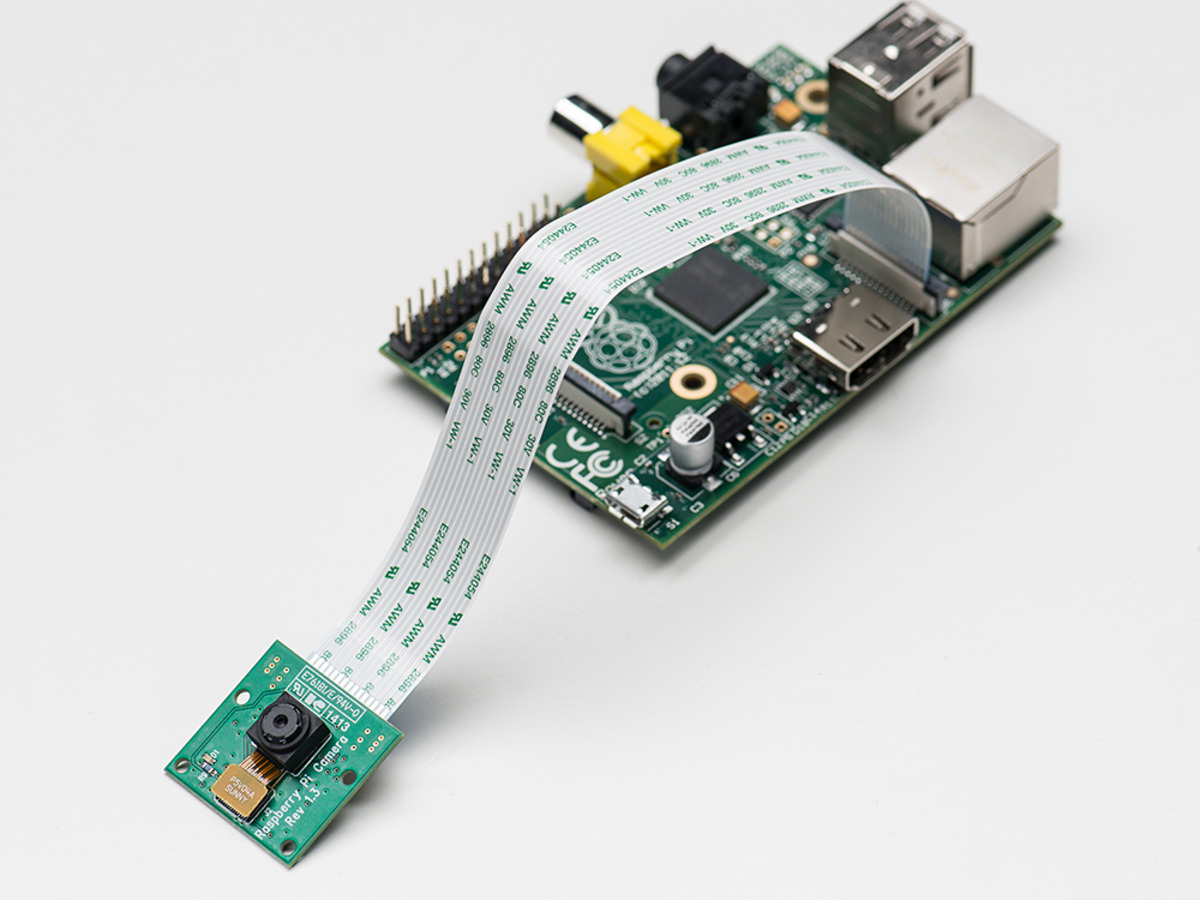
\includegraphics[width=.8\textwidth]{RaspberryPi}
  \caption{Raspberry Pi with camera module attached}
  \label{fig:raspi}
\end{figure}

The Raspberry Pi is a low cost, credit-card sized computer developed in the UK by the Raspberry Pi Foundation. The primary objective of the Raspberry Pi is to increase, and encourage the teaching of computer science in schools. In this regard it has been highly successful and since its launch in February 2012 it has sold over 2 million units~\cite{2mil}, however its success has also been, in part, due to the hobbyist and scientific markets. The Raspberry Pi boasts a 700MHz ARMv6k, 512 MB of RAM and a full Linux operating system for \$35~\cite{Broadcom-BCM2835-Website}. In addition, the Raspberry Pi foundation have released a camera module that supports up to 1080p30 video capture, and can be seen in Figure~\ref{fig:raspi}. All of these features make the Raspberry Pi an ideal candidate for imaging and image processing on a low budget.

Optical flow is the apparent motion of objects in a scene due to relative motion between an observer and the objects being observed as seen in Figure~\ref{fig:opticalflow}. It is a critical tool in many experimental methods such as Particle Image Velocimetry~\cite{quenot1998particle} for flow analysis and and soil mechanics, speckle tracking echocardiography~\cite{speckle} in medical imaging, as well as mechanical testing~\cite{harris2012characterizing}. There already exist commercial packages for executing optical flow algorithms, however licenses can often be costly and the software can require high end hardware. This project, as part of the OpenLabTools initiative, aims to provide access to optical flow methods on low cost and low powered hardware. The main objectives for the project are to:

\begin{itemize}
  \item Provide access to optical flow methods on cheap and readily available hardware
  \item Perform online and offline processing using the Raspberry Pi
  \item Capture data using the Raspberry Pi Camera
  \item Integrate with existing experiments and other OpenLabTools projects
  \item Provide a clear set of instructions aimed at undergraduate level
\end{itemize}

\begin{figure}[htpb]
  \centering
  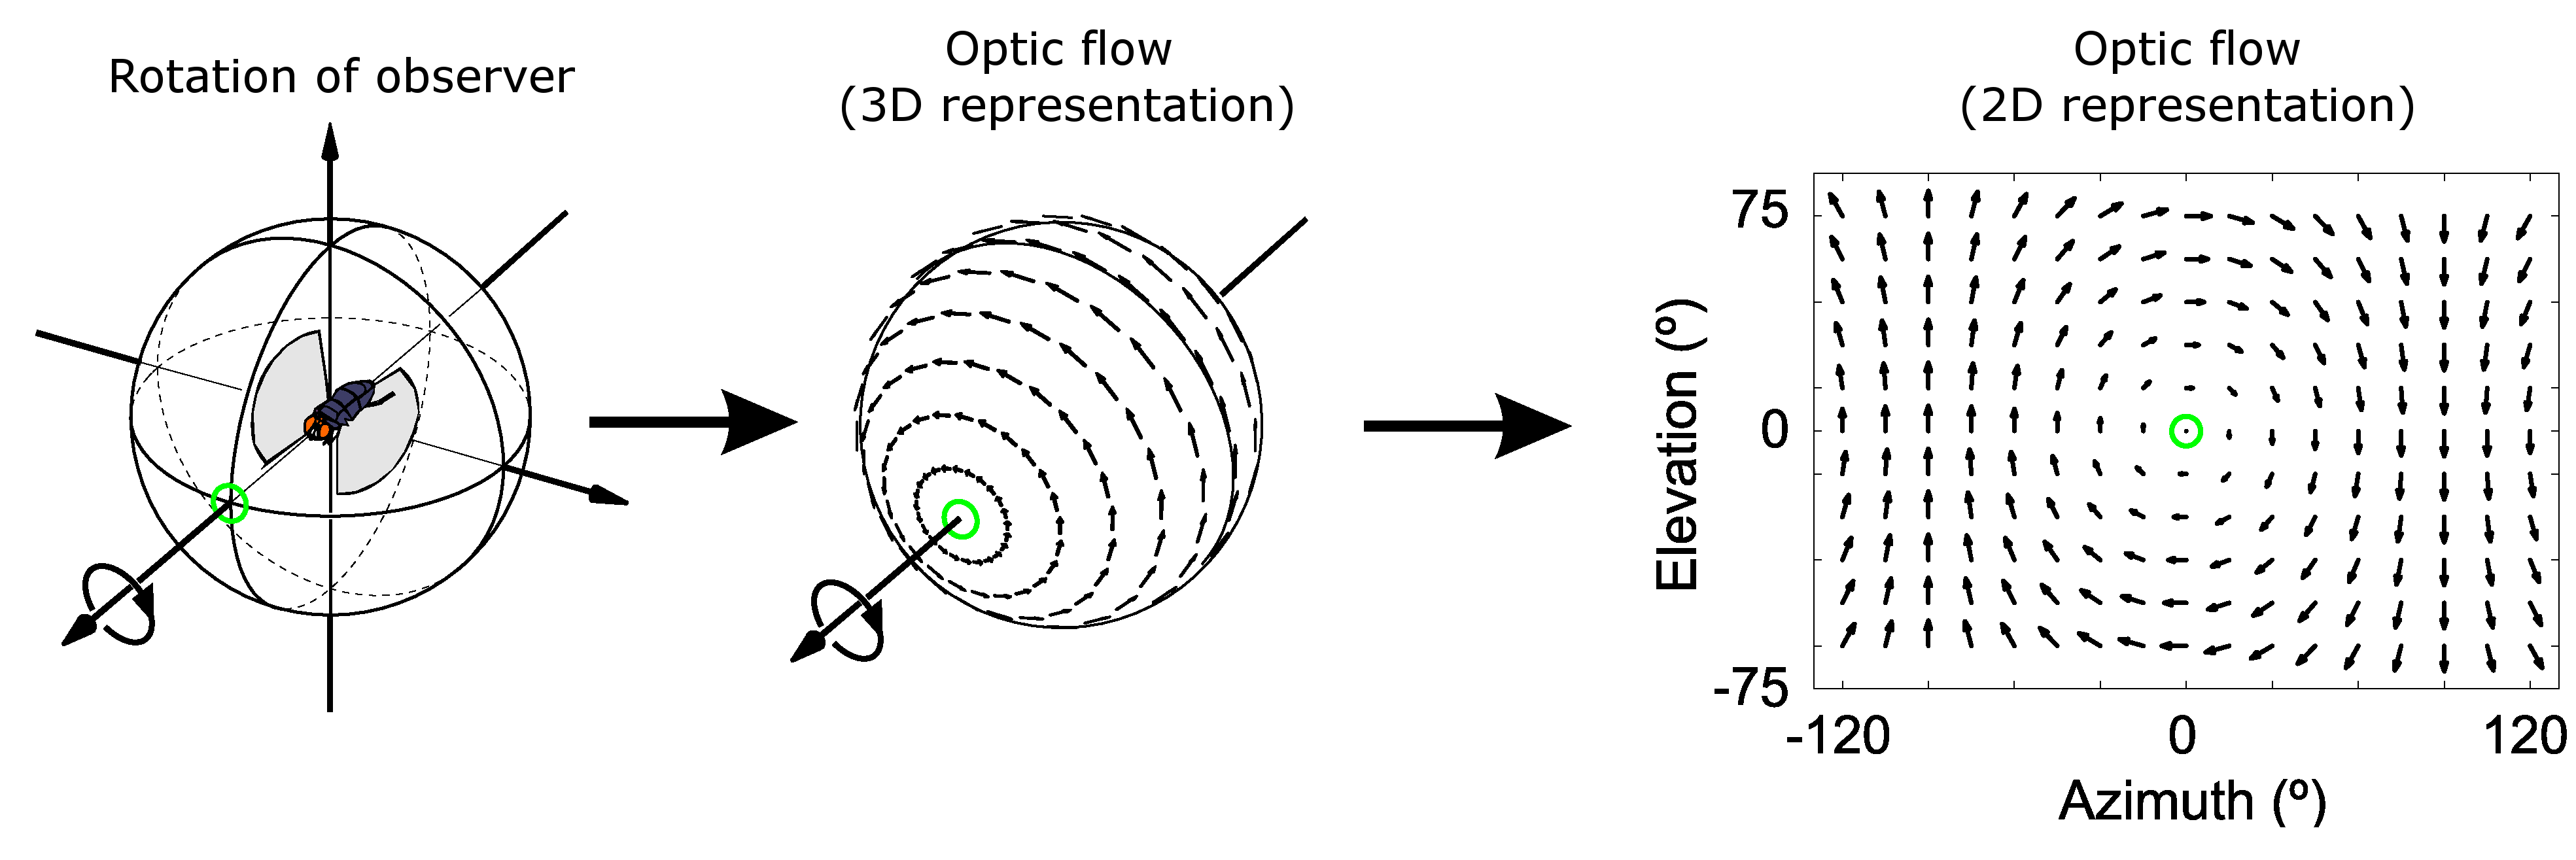
\includegraphics[width=\textwidth]{Opticfloweg}
  \caption{Optical flow caused by a rotating observer~\cite{huston2008visuomotor}}
  \label{fig:opticalflow}
\end{figure}

In section \ref{sec:theory}, \nameref{sec:theory}, I will explain the assumptions behind the theoretical development and the application of the theory. Section \ref{sec:apparatus}, \nameref{sec:apparatus}, describes the tools used in the running of the experiments and discusses the experimental accuracy. Section \ref{sec:results}, \nameref{sec:results}, presents the results obtained from the various different experiments and analyses the raw data. Finally,  section \ref{sec:conclusions}, \nameref{sec:conclusions}, highlights the main results and outlines avenues for further work and development.